\documentclass[9pt]{beamer}

\usepackage[T1]{fontenc}
\usepackage{color}
\usepackage{graphicx}
\usepackage{natbib}
\usepackage{tikz}
\usepackage{pgfgantt}

\usetheme{Boadilla}

\definecolor{rd}{HTML}{2F2A40}
\definecolor{methods}{HTML}{C6C6C6}
\definecolor{research}{HTML}{8F84BE}
\definecolor{skills}{HTML}{7A7A7A}
\definecolor{rc}{HTML}{AC152A} 

\usefonttheme{professionalfonts}

\title[Climate Topography]{A Topography of Climate Change Research}
\subtitle{}
\author{Max Callaghan}
\institute[MCC]{
	
\includegraphics[height=1cm,width=2cm]{MCC_Logo_RZ_rgb.jpg}
%	\,
%	
\includegraphics[height=1cm]{hertie_logo.png}
}

\newtheorem*{remark}{}

\bibliographystyle{apalike}

\begin{document}
	
\begin{frame}
	\titlepage
\end{frame}

\addtobeamertemplate{frametitle}{}{%
	\begin{tikzpicture}[remember picture,overlay]
	\node[anchor=north east,yshift=2pt] at (current page.north east) {
\includegraphics[height=0.8cm]{MCC_Logo_RZ_rgb.jpg}};
	\end{tikzpicture}}

\begin{frame}{Context}

\begin{columns}
	\begin{column}{0.5\linewidth}
		\begin{center}
		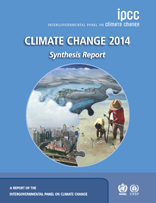
\includegraphics[width=0.6\linewidth]{syrcover.png}
		\end{center}
	\end{column}
	\begin{column}{0.5\linewidth}
	\begin{center}
		\begin{itemize}
			\item To contribute evidence-based policy-making on climate change, the IPCC aims to \textit{comprehensively} assess  
			\item These assessments should be aim to balance legitimacy, credibility and relevance \citep{Cash2001}
		\end{itemize}
	\end{center}
	\end{column}
	\end{columns}

\end{frame}

\begin{frame}{Motivation}

\begin{columns}
	\begin{column}{0.5\linewidth}
		\begin{center}
%			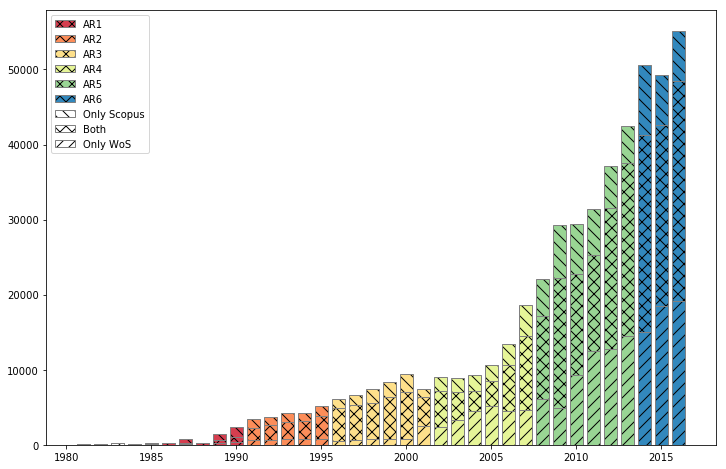
\includegraphics[width=0.85\linewidth]{../plots/wos_scopus_docs_time.png}
\begin{figure}
	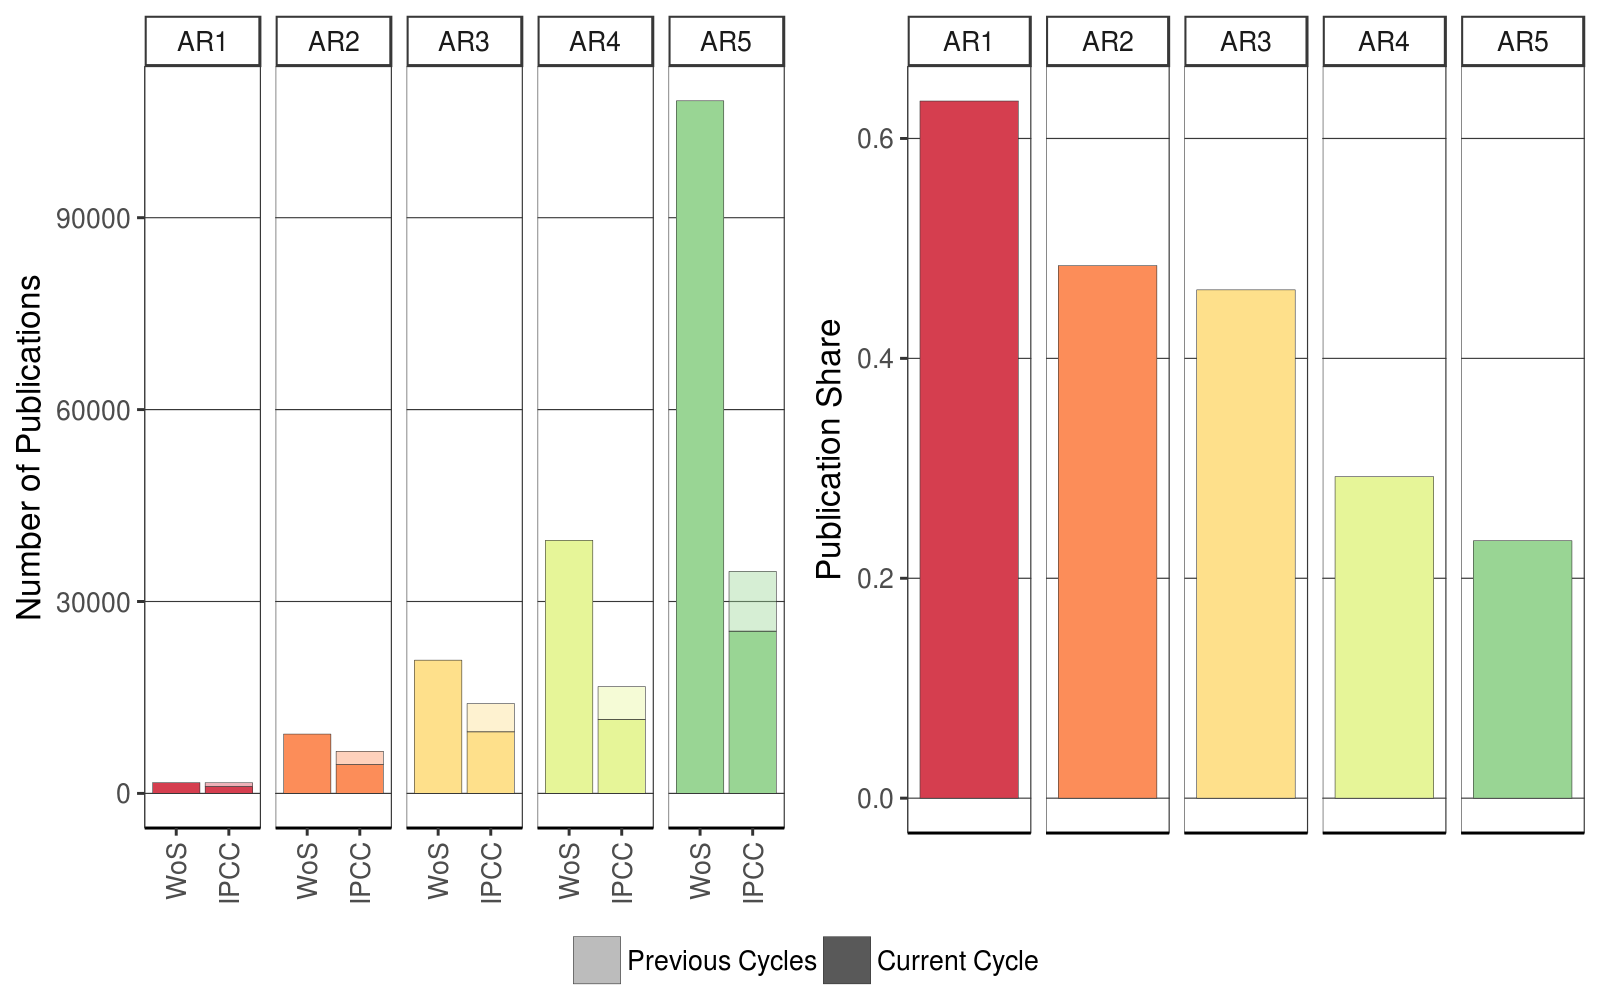
\includegraphics[width=0.85\linewidth]{merged_IPCC_spectral.png}
	\caption{Source: \citet{Minx2017l} }
\end{figure}
		\end{center}
	\end{column}
	\begin{column}{0.5\linewidth}
		\begin{center}
			\begin{itemize}
				\item Comprehensive, credible and relevant assessments become
				more challenging as the literature grows
			\end{itemize}
		\begin{remark}[]
			To understand, and to aid, scientific assessments of climate change, we need to machine read the literature
		\end{remark}
		\end{center}
	\end{column}
\end{columns}

\end{frame}

\begin{frame}{Approach - Words, words, words}

\begin{columns}
	\begin{column}{0.5\linewidth}
		\begin{center}
			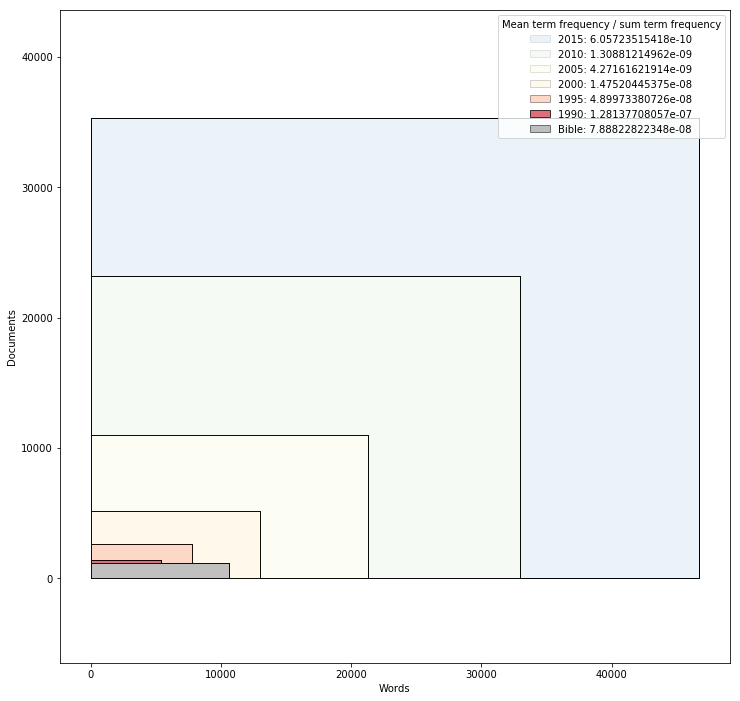
\includegraphics[width=\linewidth]{volume_variety_bible.png}
		\end{center}
	\end{column}
	\begin{column}{0.5\linewidth}
		\begin{center}
			\begin{itemize}
				\item Topic modelling is a way of reducing the dimensionality of a corpus of documents
				\item A large matrix of documents x words is factorised by
				a matrix of topics x words and a matrix of topics x documents
			\citep{Lee1999}
				\item Topics describe the latent structure of the document corpus
				
			\end{itemize}
		\end{center}
	\end{column}
\end{columns}

\end{frame}

\begin{frame}{Approach - Words, words, words}

\begin{figure}
	
	\[V_{i\mu} \]
	
	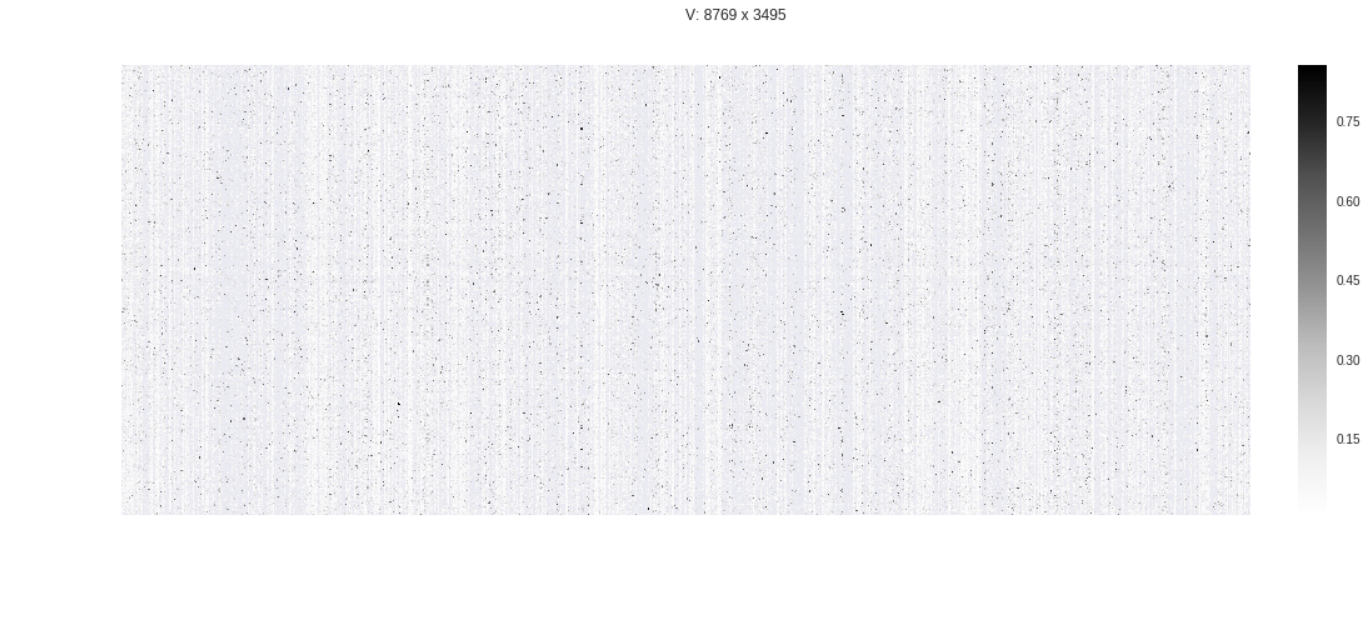
\includegraphics[width=\linewidth]{../plots/VWH_blank.png}
	
	\caption{A topic model of 3495 documents on climate change from the year 2000}
	
\end{figure}

\end{frame}


\begin{frame}{Approach - Words, words, words}

\begin{figure}
	
	\[V_{i\mu} \approx (WH)_{i\mu} = \sum_{a=1}^{r}W_{ia}H_{a\mu} \]
	
	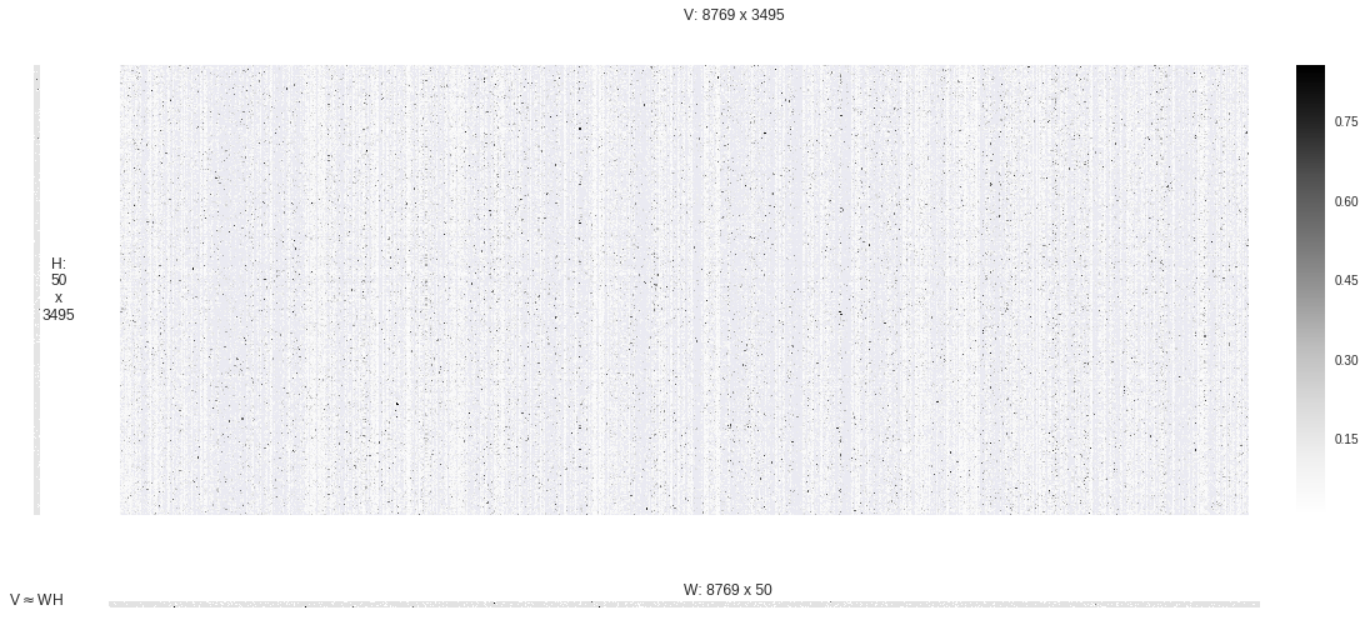
\includegraphics[width=\linewidth]{../plots/VWH.png}
	
	\caption{A topic model of 3495 documents on climate change from the year 2000}
	
\end{figure}


\end{frame}

\begin{frame}{Research Questions}
\begin{itemize}
	\item What topics are discovered endogenously from a corpus of > 200,000 abstracts on climate change?
	\item How do these topics describe the structure of the literature?
	\item Which topics have grown recently?
	\item Which topics are better and less well represented in IPCC assessment reports?
\end{itemize}

\end{frame}


\begin{frame}{Preliminary results - explanation}

\begin{columns}
	\begin{column}{0.5\linewidth}
		\begin{center}
			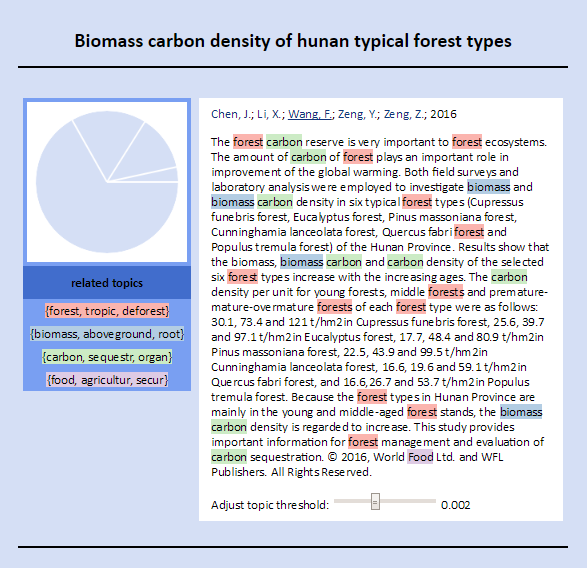
\includegraphics[width=\linewidth]{../plots/biomass_eg.png}
		\end{center}
	\end{column}
	\begin{column}{0.5\linewidth}
		\begin{center}
			\begin{itemize}
				\item Documents are mixtures of topics, based on the words which occur in them
			\end{itemize}
		\end{center}
	\end{column}
\end{columns}

\end{frame}


\begin{frame}{Preliminary results - structure}

\begin{columns}
	\begin{column}{0.65\linewidth}
		\begin{center}	
			\vspace*{-0.1\linewidth}
			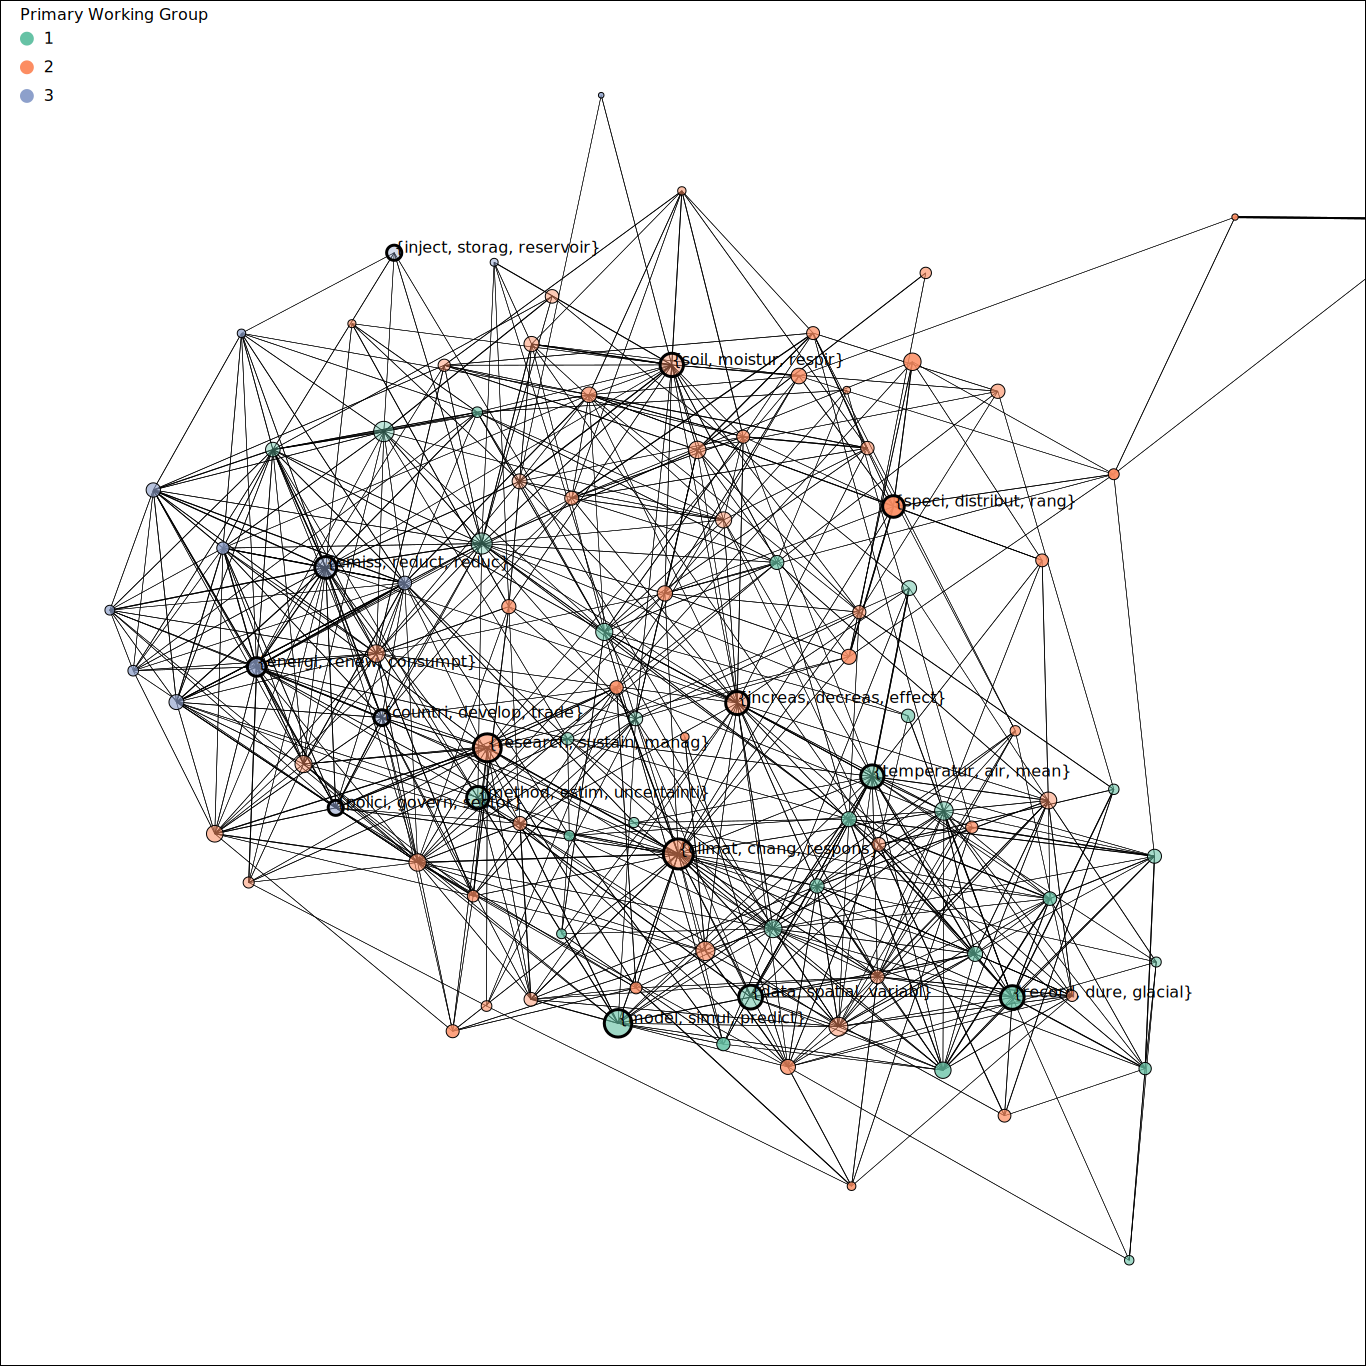
\includegraphics[width=1.1\linewidth]{../plots/network_wg_372.PNG}
		\end{center}
	\end{column}
	\begin{column}{0.35\linewidth}
		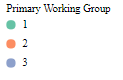
\includegraphics[width=0.4\linewidth]{../plots/network_wg_key.PNG}
		\begin{center}
			\begin{itemize}
				\item A network of comprehensible topics is generated with 100 topics
				\item Topics can be matched to the IPCC working group from which the majority of the topic documents are referenced in
				\item Topics from the same working group are \textbf{significantly} more likely to be correlated with each other than those which are not
			\end{itemize}
		\end{center}
	\end{column}
\end{columns}

\end{frame}

\begin{frame}{Preliminary results - structure - WGI}

\begin{columns}
	\begin{column}{0.65\linewidth}
		\begin{center}
			\vspace*{-0.1\linewidth}
			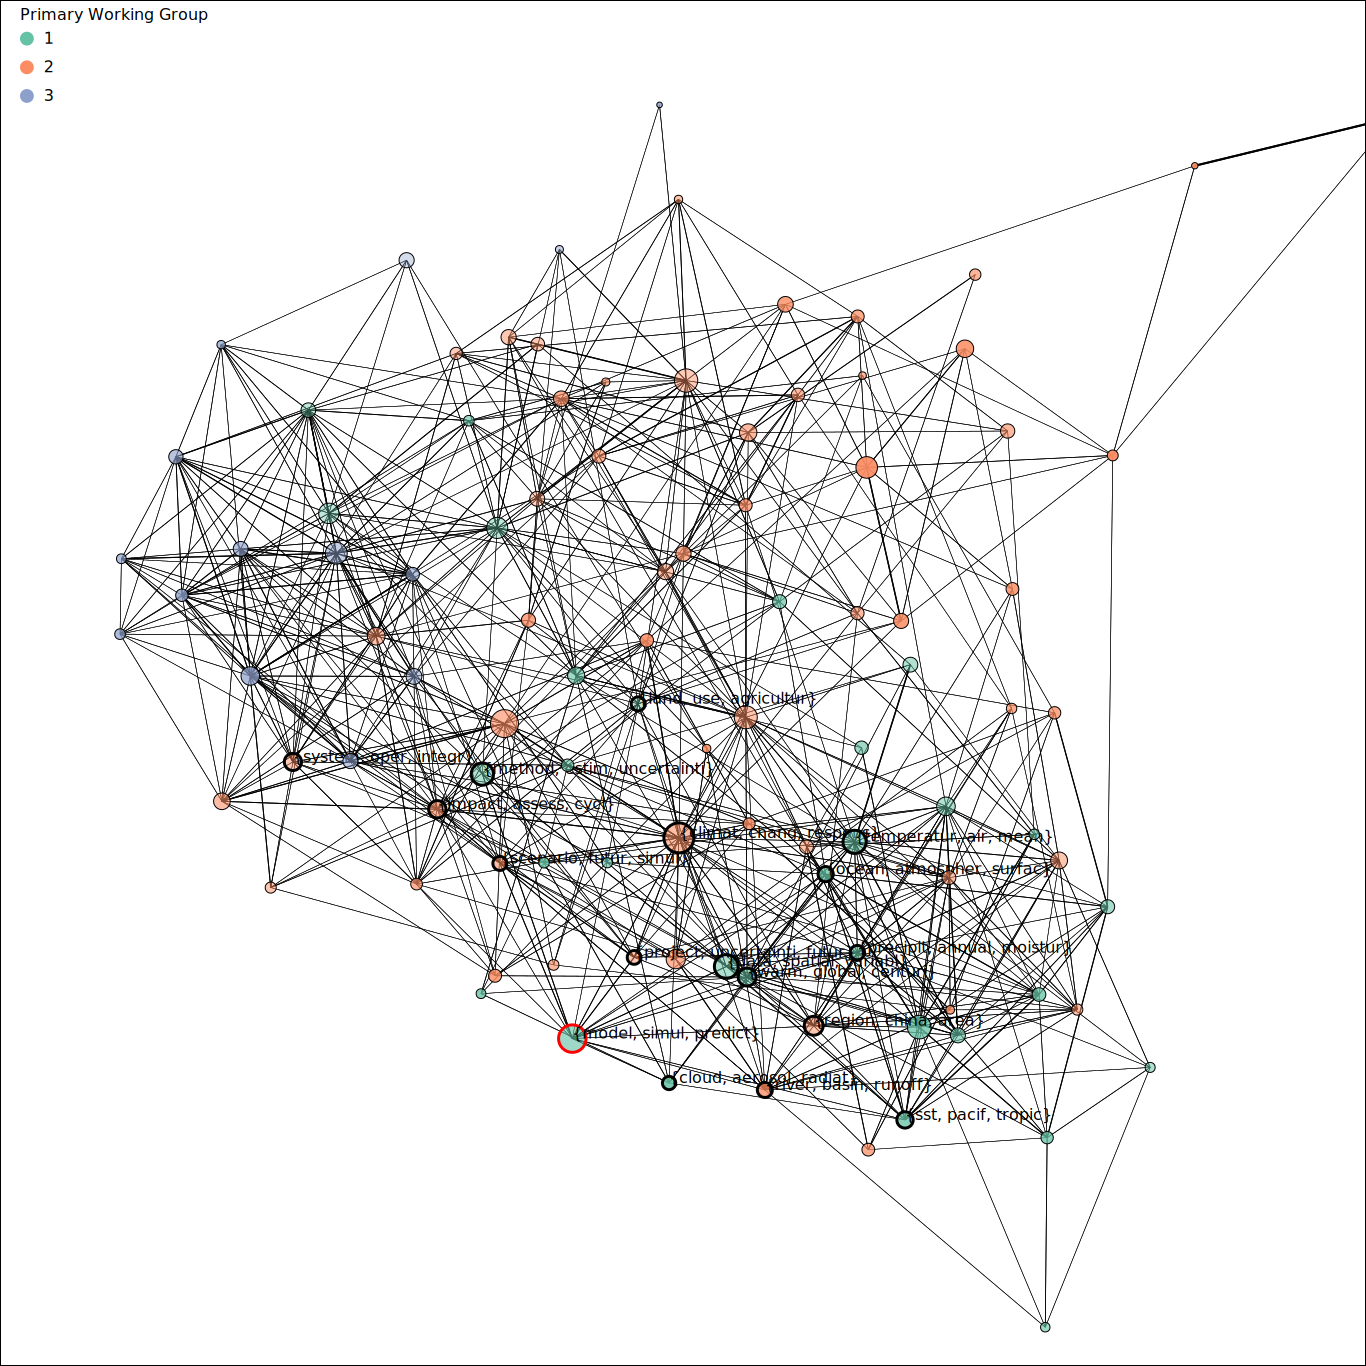
\includegraphics[width=1.1\linewidth]{../plots/network_wg_372_1.PNG}
		\end{center}
	\end{column}
	\begin{column}{0.35\linewidth}
		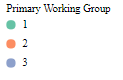
\includegraphics[width=0.4\linewidth]{../plots/network_wg_key.PNG}
		\begin{center}
			\begin{itemize}
				\item The largest topic in WGI is on models.
			\end{itemize}
		\end{center}
	\end{column}
\end{columns}

\end{frame}

\begin{frame}{Preliminary results - structure - WGII}

\begin{columns}
	\begin{column}{0.65\linewidth}
		\begin{center}
			\vspace*{-0.1\linewidth}
			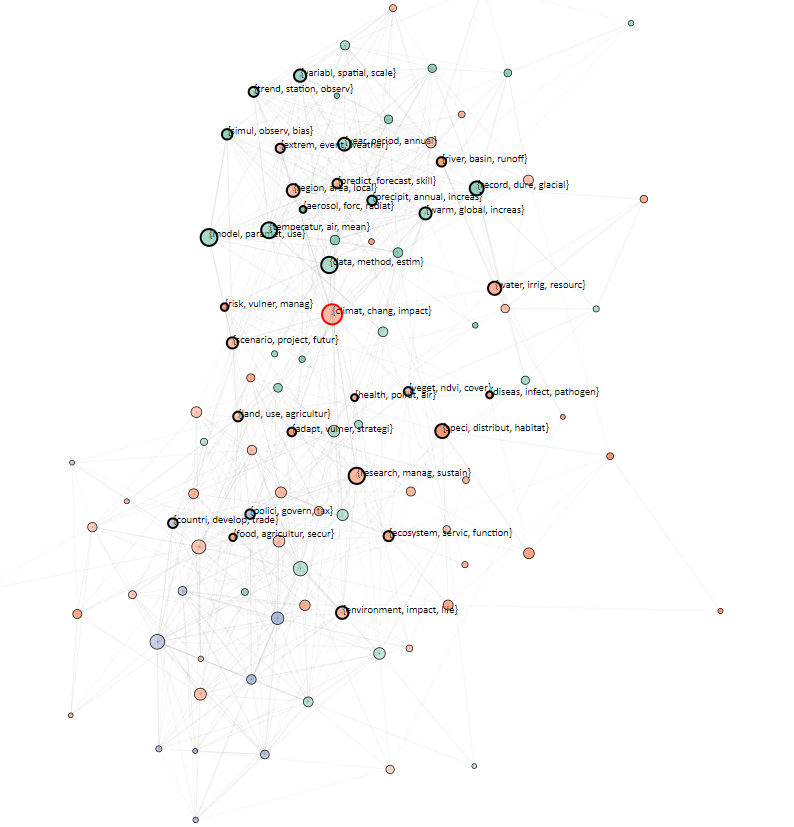
\includegraphics[width=1.1\linewidth]{../plots/network_wg_372_2.PNG}
		\end{center}
	\end{column}
	\begin{column}{0.35\linewidth}
		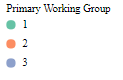
\includegraphics[width=0.4\linewidth]{../plots/network_wg_key.PNG}
		\begin{center}
			\begin{itemize}
				\item The largest primarily WGII topic is on climate change impacts
			\end{itemize}
		\end{center}
	\end{column}
\end{columns}

\end{frame}

\begin{frame}{Preliminary results - structure - WGIII}

\begin{columns}
	\begin{column}{0.65\linewidth}
		\begin{center}
			\vspace*{-0.1\linewidth}
			
\includegraphics[width=1.1\linewidth]{../plots/network_wg_372_3.PNG}
		\end{center}
	\end{column}
	\begin{column}{0.35\linewidth}
		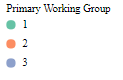
\includegraphics[width=0.4\linewidth]{../plots/network_wg_key.PNG}
		\begin{center}
			\begin{itemize}
				\item The largest WGIII topic is on emissions reductions.
			\end{itemize}
		\end{center}
	\end{column}
\end{columns}

\end{frame}

\begin{frame}{Preliminary results - structure - other clusters}

\begin{columns}
	\begin{column}{0.65\linewidth}
		\begin{center}
			\vspace*{-0.1\linewidth}
			\hspace*{-0.1\linewidth}
			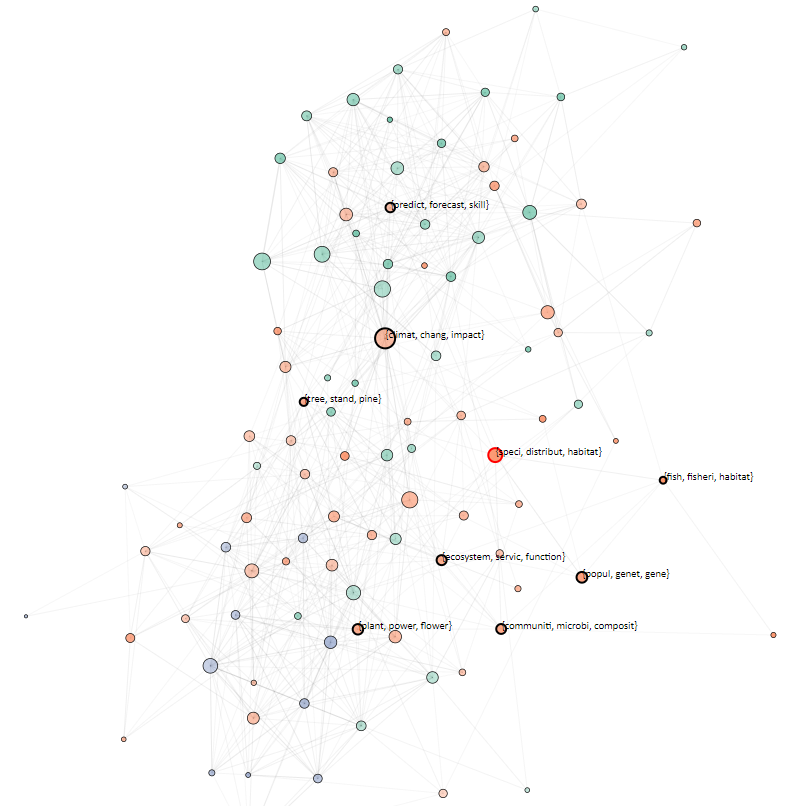
\includegraphics[width=1.25\linewidth]{../plots/network_wg_372_4.PNG}
		\end{center}
	\end{column}
	\begin{column}{0.35\linewidth}
		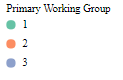
\includegraphics[width=0.4\linewidth]{../plots/network_wg_key.PNG}
		\begin{center}
			\begin{itemize}
				\item A fourth cluster of mostly WGII references contains topics on ecosystems, species and habitats
			\end{itemize}
		\end{center}
	\end{column}
\end{columns}

\end{frame}

\begin{frame}{Preliminary results - structure}

\begin{columns}
	\begin{column}{0.6\linewidth}
		\begin{center}			
			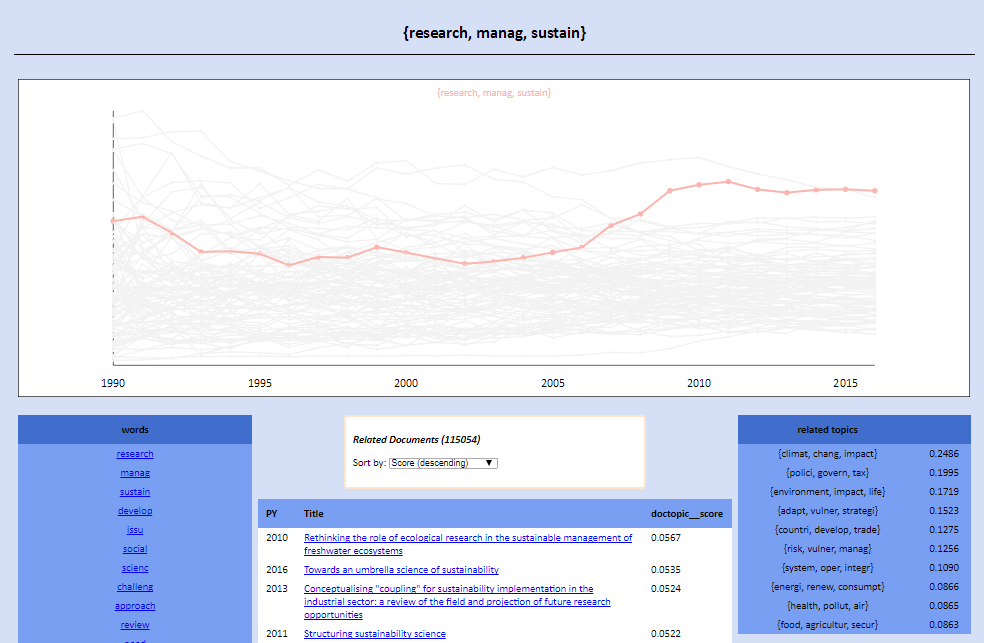
\includegraphics[width=\linewidth]{../plots/sustainability.PNG}
		\end{center}
	\end{column}
	\begin{column}{0.4\linewidth}
		\begin{center}
			\begin{itemize}
				\item In later assessment periods, a large meta-topic on research priorities and sustainability emerges
			\end{itemize}
		\end{center}
	\end{column}
\end{columns}

\end{frame}

\begin{frame}{Preliminary results - growth}

\begin{columns}
	\begin{column}{0.6\linewidth}
		\begin{center}
			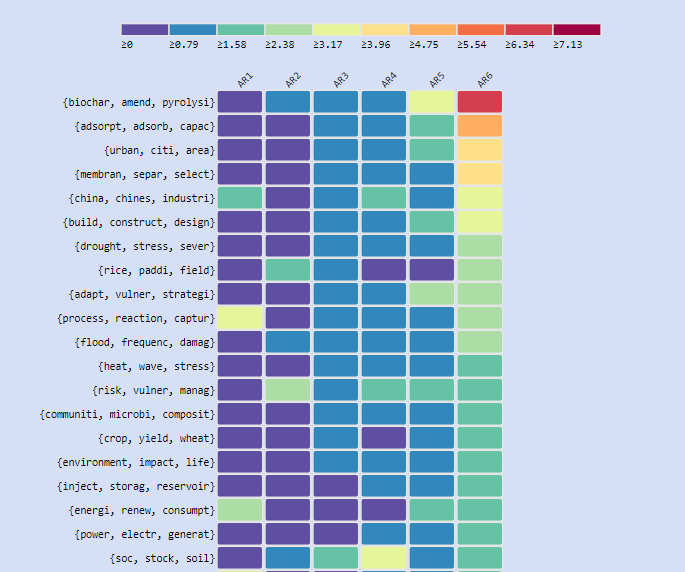
\includegraphics[width=\linewidth]{../plots/top_20_386.png}
		\end{center}
	\end{column}
	\begin{column}{0.4\linewidth}
		\begin{center}
			\begin{itemize}
				\item Negative emissions related topics have shown strong growth since the end of AR5
				\item As have topics on cities and extreme weather events
			\end{itemize}
		\end{center}
	\end{column}
\end{columns}

\end{frame}

\begin{frame}{Preliminary results - growth - biochar}


		\begin{center}
			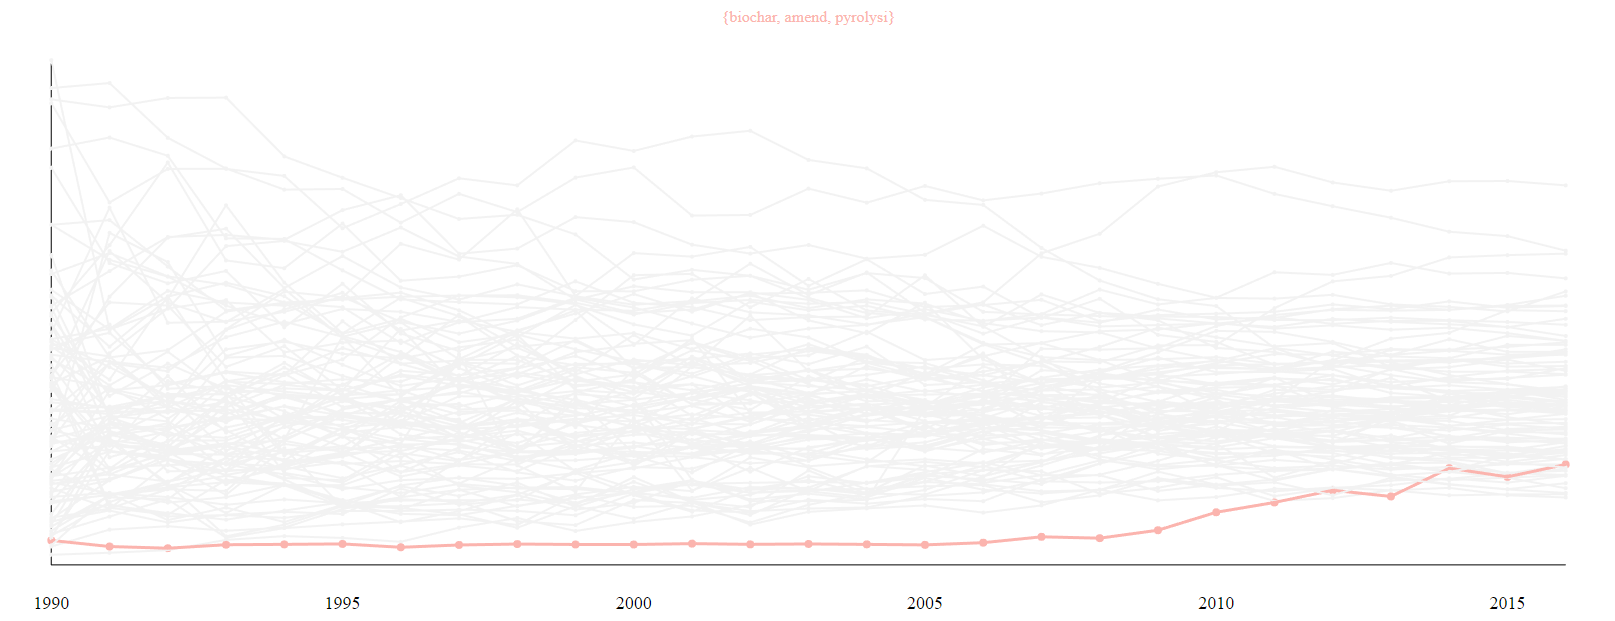
\includegraphics[width=\linewidth]{../plots/biochar_growth.png}

		\medskip

			\begin{itemize}
				\item Biochar has emerged as an entirely new topic in the last 10 years
			\end{itemize}
		\end{center}

\end{frame}

\begin{frame}{Preliminary results - gaps in coverage}

How can we get a sense of which topics are better covered in IPCC reports?

\begin{itemize}
	\item Each document \(d\) either matches or does not match an IPCC reference
	\item For each topic \(h\), we can sum the scores for each category of document
	\item The ``IPCC proportion'' of each topic is the proportion of the sum of the document score accounted for by documents which match IPCC references.
\end{itemize}



\end{frame}

\begin{frame}{Preliminary results - gaps in coverage}

\begin{columns}
	\begin{column}{0.7\linewidth}
		\begin{center}
			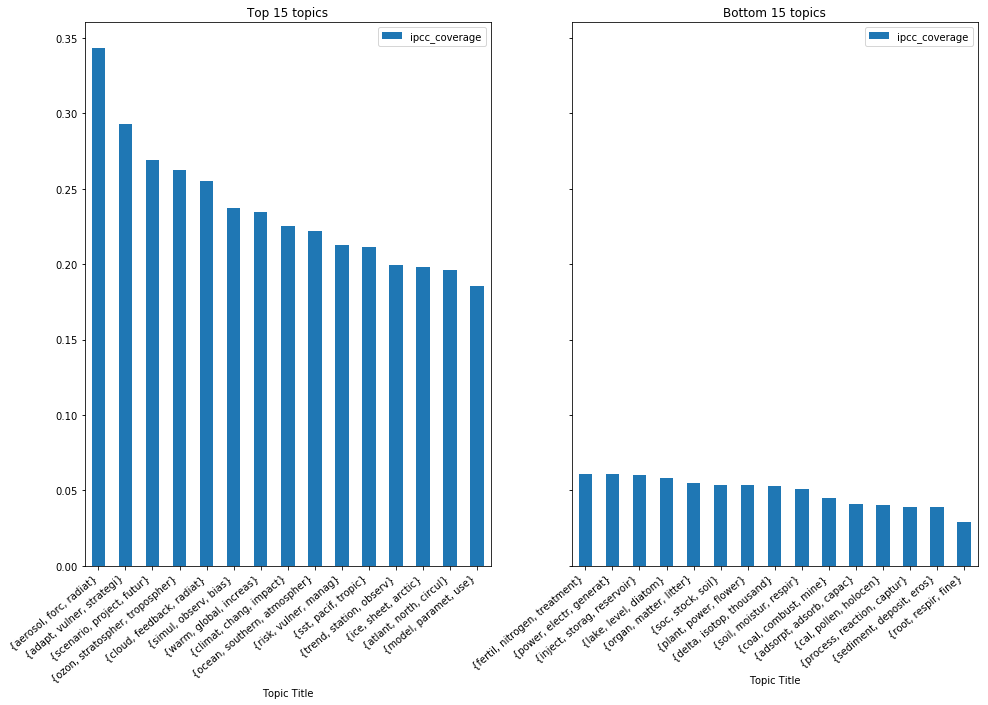
\includegraphics[width=\linewidth]{../plots/ipcc_topics_386.png}
		\end{center}
	\end{column}
	\begin{column}{0.3\linewidth}
		\begin{center}
			\begin{itemize}
				\item The physical science aspects of climate change, as well topics on impacts, adaptation and scenarios are well covered by the IPCC
				\item Topics on specific technological solutions (particularly NETs), as well as soils, are less well covered
			\end{itemize}
		\end{center}
	\end{column}
\end{columns}

\end{frame}

\begin{frame}{Conclusions}


\begin{itemize}
	\item Endogenously discovered topics make substantive sense of an unmanageable dataset of climate-relevant literature
	\item Topic modelling discovers over-arching topics such as that on sustainability and research priorities, as well as individual, fast growing topics such as biochar or CCS
	\item Topics from the same IPCC working group are more likely to be connected to each other.
	\item Quantitative evidence is found to support policy makers' dissatisfaction with a lack of `solution orientation' in IPCC reports \citep{Kowarsch2017} 
\end{itemize}

\end{frame}


\begin{frame}{Extra results - Journals}

\begin{columns}
	\begin{column}{0.55\linewidth}
		\begin{center}
			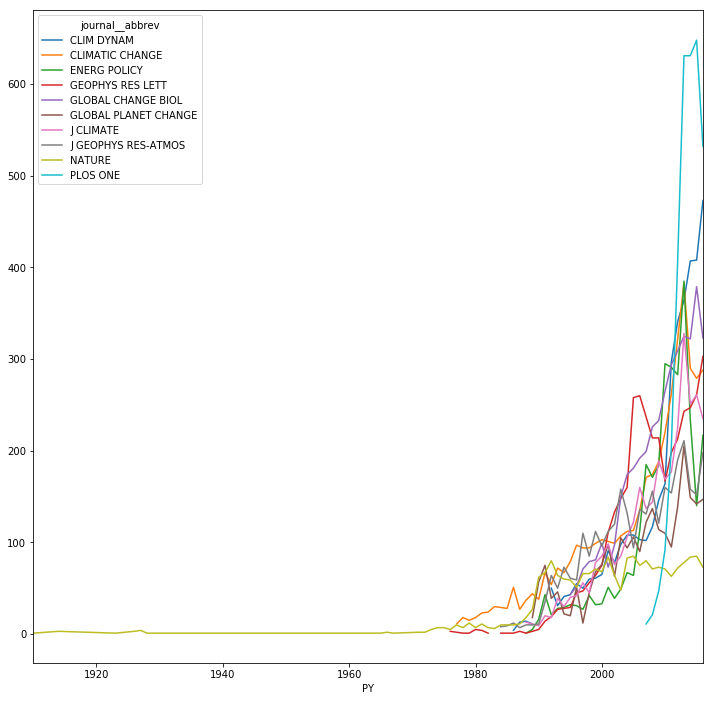
\includegraphics[width=\linewidth]{../plots/journals/journal_papers.png}
		\end{center}
	\end{column}
	\begin{column}{0.45\linewidth}
		\begin{center}
			\begin{itemize}
				\item Nature has been publishing about climate change for a long time
				\item Plos One has very recently overtaken all other journals
				\item The number of journals has risen very steeply
			\end{itemize}
		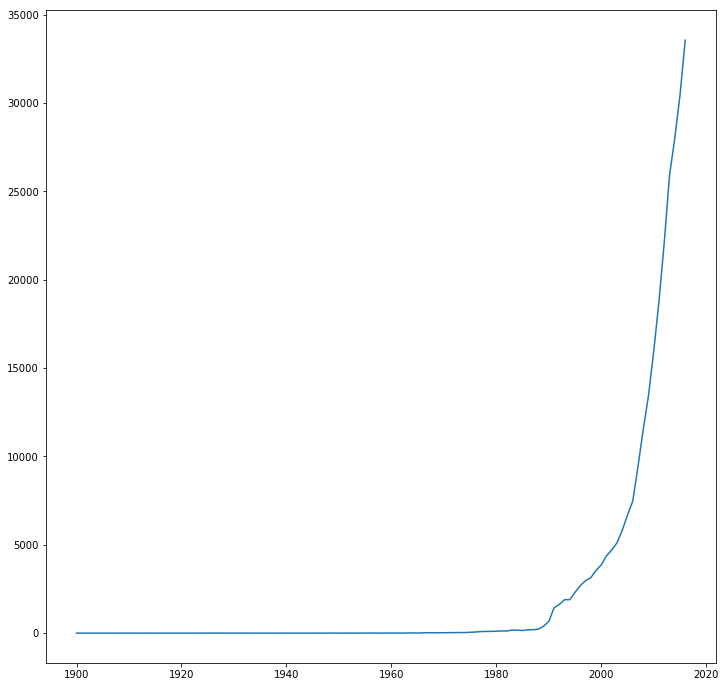
\includegraphics[width=0.9\linewidth]{../plots/journals/n_journals.png}
		\end{center}
	\end{column}
\end{columns}

\end{frame}

\begin{frame}{Extra results - Journals}

\begin{columns}
	\begin{column}{0.55\linewidth}
		\begin{center}
			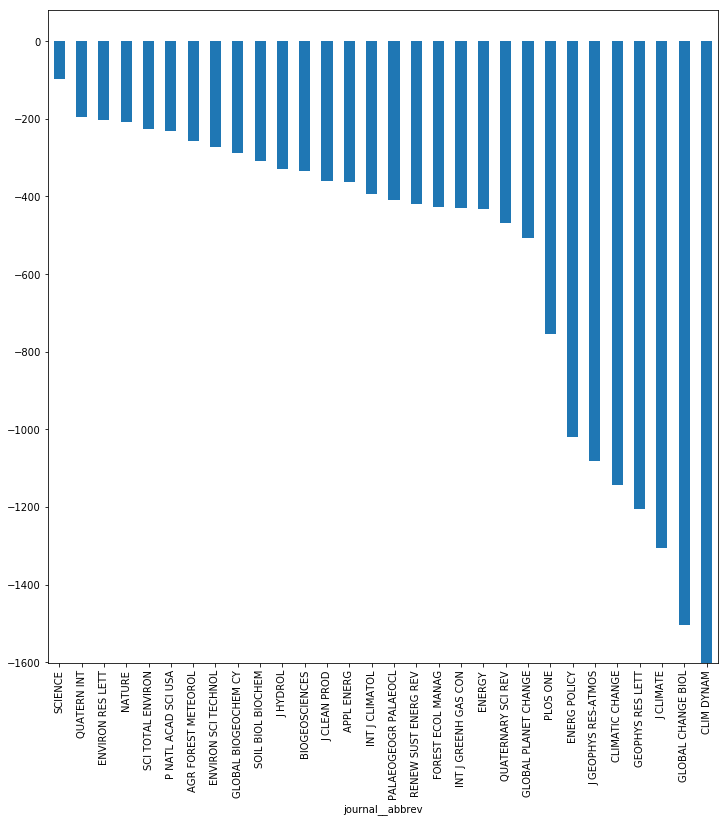
\includegraphics[width=\linewidth]{../plots/journals/journal_entropy_386.png}
		\end{center}
	\end{column}
	\begin{column}{0.45\linewidth}
		\begin{center}
			\begin{itemize}
				\item Journal Entropy describes the distribution of topics in a journal \citep{Hall2008a}
				\item High values mean the journal deals with a wider range of topics
			\end{itemize}
			\[  H(z\rvert c,y) = -\sum_{i=1}^{K} \hat{p}(z_i \rvert c,y) \; log \; \hat{p}(z_i \rvert c, y) \]
		\end{center}
	\end{column}
\end{columns}

\end{frame}

\begin{frame}{Extra results - Journals}

	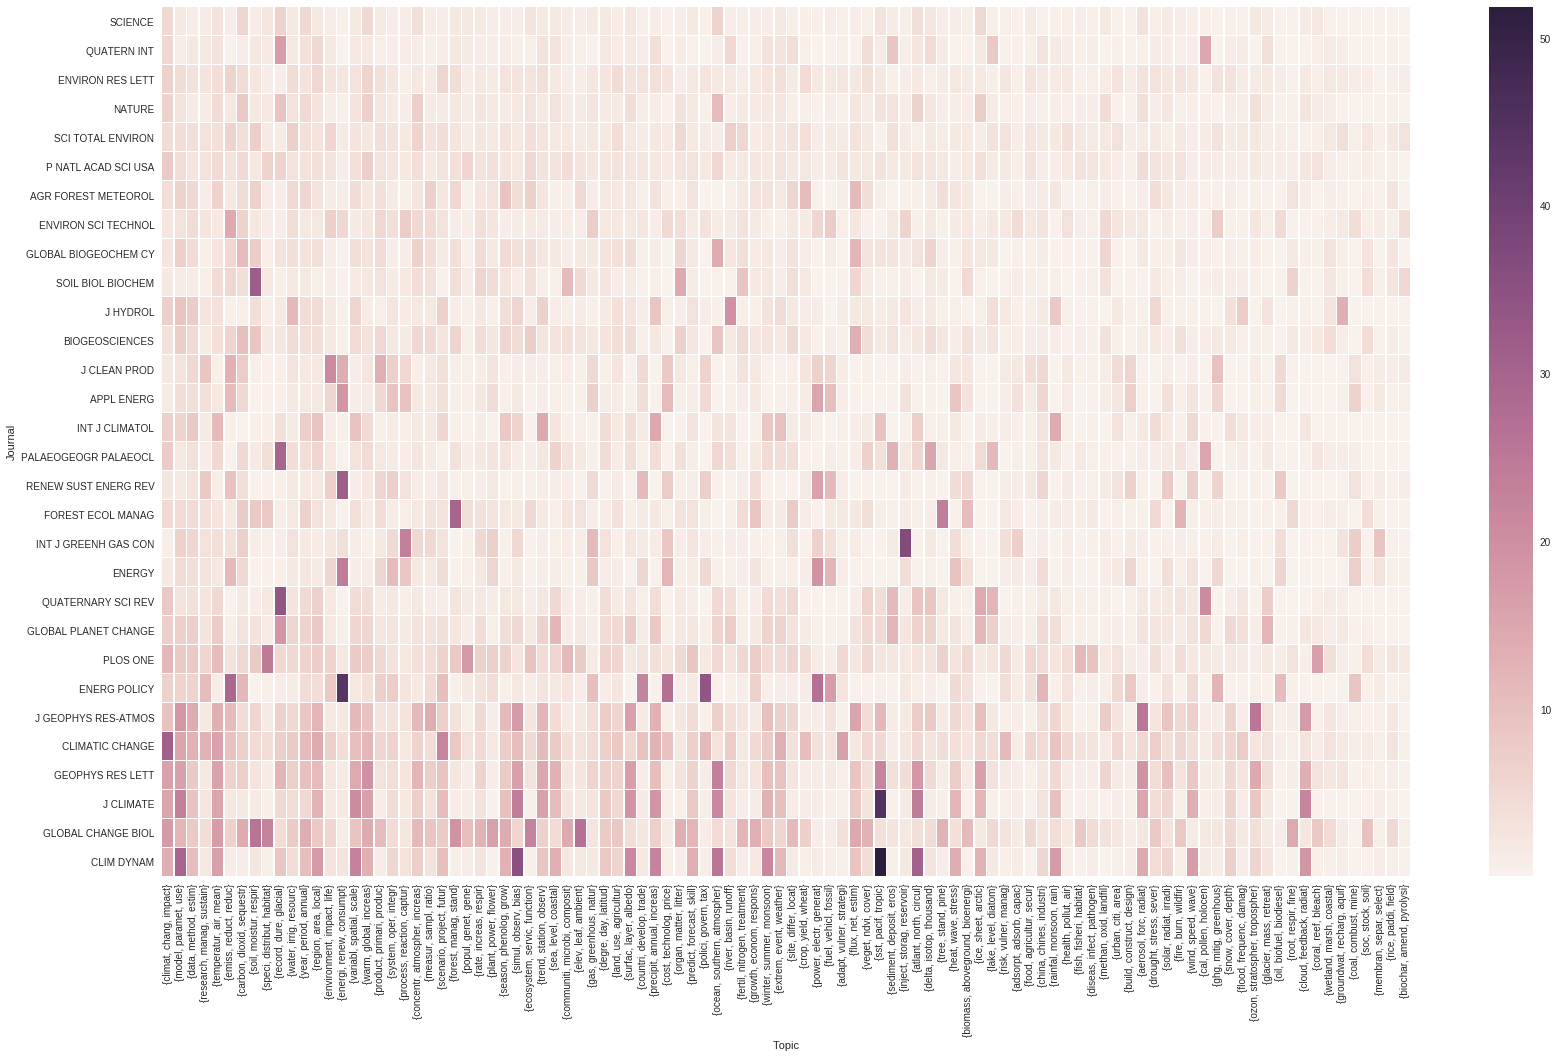
\includegraphics[width=\linewidth]{../plots/journals/journal_topics_386.png}

\end{frame}


%\begin{frame}{Outlook}
%
%\begin{figure}
%
%\tiny
%
%\begin{ganttchart}[
%	y unit title=0.3cm,
%	y unit chart=0.5cm,
%	x unit= 0.2cm,
%	vgrid,hgrid,
%	vgrid={{dotted,dotted,black}},
%	title height=1,
%	%     title/.style={fill=none},
%	title label font=\bfseries\scriptsize,
%	%bar/.style={fill=blue},
%	bar height=0.7,
%	bar label font=\tiny,
%	%   progress label text={},
%	group right shift=0,
%	group top shift=0.7,
%	group height=.3,
%	group peaks width={0.2},
%	inline]{1}{42}
%	\gantttitle{2017}{9}
%	\gantttitle{2018}{12}
%	\gantttitle{2019}{12}
%	\gantttitle{2020}{9} \\
%	\gantttitlelist{2,...,4}{3} \gantttitlelist{1,...,4}{3} \gantttitlelist{1,...,4}{3} \gantttitlelist{1,...,3}{3} \\
%	\gantttitlelist{4,...,12}{1} \gantttitlelist{1,...,12}{1}
%	%\gantttitlelist{J,F,M,A,M,J,J,A,S,O,N,D}{1}
%	\gantttitlelist{1,...,12}{1} \gantttitlelist{1,...,9}{1}\\
%	
%	% HERTIE
%	\ganttgroup[inline=false]{Hertie Courses}{6}{42} \\
%	
%	\ganttbar[inline=false, bar/.append style={fill=rd}]{Research Design}{6}{15} \\
%	\ganttbar[inline=false, bar/.append style={fill=methods}]{Methods}{6}{15} \\
%	\ganttbar[inline=false, bar/.append style={fill=skills}]{Skills}{6}{15} \\
%	\ganttbar[inline=false, bar/.append style={fill=rc}]{Research Colloquium}{19}{42} \\
%	
%	% HERTIE
%	\ganttgroup[inline=false]{Thesis Research}{1}{42} \\
%	\ganttbar[inline=false, bar/.append style={fill=research}]{Knowledge Map}{1}{5} \\
%	\ganttbar[inline=false, bar/.append style={fill=research}]{Pyramid}{6}{15} \\
%	
%	
%	\ganttbar[inline=false, bar/.append style={fill=research}]{Knowledge Accumulation}{16}{27} \\
%	
%	\ganttbar[inline=false, bar/.append style={fill=research}]{Evidence in Policy}{19}{27} \\
%	
%	\ganttbar[inline=false, bar/.append style={fill=research}]{Envelope}{28}{33} \\
%	
%	\ganttbar[inline=false, bar/.append style={fill=research}]{Revisions/Contingency}{34}{42} \\
%	
%	%\ganttlinkedbar[inline=false]{Task 2}{3}{7} \ganttnewline
%	%\ganttmilestone[inline=false]{Milestone}{7} \ganttnewline
%	
%	
%	
%\end{ganttchart} 
%
%\end{figure}
%
%\end{frame}



\begin{frame}{Frame Title}
	\small
	\bibliography{C:/Users/galm/Documents/library/library}
\end{frame}

\end{document}
